\documentclass[12pt,fleqn]{article}
\usepackage{a4}
\usepackage{graphicx}
\usepackage{psfrag}
\usepackage{amsmath}                     % \boldsymbol{#1}
\usepackage{amssymb}
%\usepackage{hangcaption}
%\usepackage{Styles/pstricks}
%\usepackage{Styles/pst-node}
\usepackage{Styles/fancyheadings}
\usepackage{tocloft}
%-----Tex width---------------------------------
\textwidth 16cm

%-----Line spacing-------------------------------
\renewcommand{\baselinestretch}{1.5}     % 1,1-zeilig

%---------Add dots in TOC-----------------------
\renewcommand{\cftsecleader}{\cftdotfill{\cftdotsep}}

%------Paragraph indention-------------------------------
\setlength{\parskip}{1.5ex plus0.5ex minus0.5ex}

%-----Prevent indent----------------------
\setlength{\parindent}{0em}

%-----Richtiger Abstand fur Einheiten-------------
\def\Unit{\hspace{0.25em}}

%-----Definition of the header--------------------
\pagestyle{fancyplain}
\renewcommand{\sectionmark}[1]{\markboth{Chapter~\thesection.~#1}{#1}}
\renewcommand{\subsectionmark}[1]{\markright{\thesubsection\ #1}}
\rhead[\fancyplain{}{\leftmark}]%
{\fancyplain{\thepage}{\thepage}} \cfoot{} \plainheadrulewidth
0.4pt
%% Otherwise: Overfull \vbox-Warning against fancyheadings-pacakage
%%  idea of: nic@minster.york.ac.uk (Nick Cropper)
\makeatletter
\ifcase \@ptsize \relax % 10pt
  \addtolength{\headheight}{1\p@}
\or % 11pt
  \addtolength{\headheight}{2\p@}
\or % 12pt
  \addtolength{\headheight}{3\p@}
\fi \makeatother

%-----Equations / Figures / Tables numbering according to \ sections
\makeatletter
\renewcommand\theequation{\thesection.\arabic{equation}}
\renewcommand\thefigure{\thesection.\arabic{figure}}
\renewcommand\thetable{\thesection.\arabic{table}}
\@addtoreset{equation}{section} \@addtoreset{figure}{section}
\@addtoreset{table}{section} \makeatother

%-----Useful abbreviations----------------------
\newcommand{\mr}{\mathrm}
\newcommand{\bs}[1]{\mbox{$\boldsymbol{#1}$}}
\newcommand{\degree}[1]{\mbox{$#1^\circ$}}

%\renewcommand{\figurename}{Bild}

%------Bibliography style-----------------------
\bibliographystyle{IEEEtran}

%-----Aufzaehlunstiefe im Literaturverzeichnis---------------
\setcounter{tocdepth}{3}

\begin{document}
\pagenumbering{Roman}
\begin{titlepage}
  \begin{center}
      \vspace*{-4.0cm}
    \begin{figure}[!h]
\centering

\includegraphics[width=0.3\linewidth]{Figures/JKUAT_logo}
%\caption{}
\label{fig:jomologo}
\end{figure}
   \large{Jomo Kenyatta University of Agriculture and Technology}\\
    %\large{College of Engineering and Technology}\\
    %\large{School of Mechanical, Materials, and Manufacturing Engineering}\\
   %\large{Department of Mechatronic Engineering}\\

    ------------------------------------------------------------------------------------------------\\[1.0cm]
    \LARGE{\textbf{Development of a Face Recognition Device to Monitor Entry Points of Institutions and Class Attendance}}\\[0.6cm]
    \LARGE{\textbf{(Otherwise called Visage)}}\\[1.5cm]
    %\large{by}\\[0.6cm
    
    ------------------------------------------------------------------------------------------------\\[1.0cm]

    \vspace{0.5cm}
    \large{\textbf{Earl Spencer Mogire
            }}\\
     \large{\textbf{Kamadi Washington Kigani
            }}\\[1.0cm]
%     \large{\textbf{Supervisors}}\\
%    \large{Dr.-Ing.~Jackson G. Njiri}\\
%    \large{Prof. George N. Nyakoe}\\
%    \large{\ldots}    \\[0.2cm]\vfill
    \large{\small{\today}}\\
    ------------------------------------------------------------------------------------------------\\[1.5cm]
  \end{center}
\end{titlepage}
%
%\pagenumbering{gobble}% Remove page numbers (and reset to 1)

%\addcontentsline{toc}{section}{Declaration}
\section*{Declaration}

We hereby declare that the work contained in this report is original; researched and documented by the undersigned students. It has not been used or presented elsewhere in any form for award of any academic qualification or otherwise. Any material obtained from other parties have been duly acknowledged. We have ensured that no violation of copyright or intellectual property rights have been committed.
\begin{enumerate}
	\item Sammy Kerata Oina\vspace*{.2cm}\\
	Signature\ldots\ldots\ldots\ldots\ldots\ldots\ldots\ldots\ldots\ldots Date\ldots\ldots\ldots\ldots\ldots\ldots\ldots\ldots\ldots\ldots
	\item Earl Spencer Mogire\vspace*{.2cm}\\
	Signature\ldots\ldots\ldots\ldots\ldots\ldots\ldots\ldots\ldots\ldots Date\ldots\ldots\ldots\ldots\ldots\ldots\ldots\ldots\ldots\ldots
\end{enumerate}

\vspace*{.5cm}
Approved by supervisors:
\begin{enumerate}
	\item Dr.-Ing. Jackson G. Njiri\vspace*{.2cm}\\
	Signature\ldots\ldots\ldots\ldots\ldots\ldots\ldots\ldots\ldots\ldots Date\ldots\ldots\ldots\ldots\ldots\ldots\ldots\ldots\ldots\ldots
	\item Prof. George N. Nyakoe\vspace*{.2cm}\\
	Signature\ldots\ldots\ldots\ldots\ldots\ldots\ldots\ldots\ldots\ldots Date\ldots\ldots\ldots\ldots\ldots\ldots\ldots\ldots\ldots\ldots
	\item Ms. Lucy W. Kariuki\vspace*{.2cm}\\
	Signature\ldots\ldots\ldots\ldots\ldots\ldots\ldots\ldots\ldots\ldots Date\ldots\ldots\ldots\ldots\ldots\ldots\ldots\ldots\ldots\ldots
\end{enumerate}



%\clearpage
%\addcontentsline{toc}{section}{Abstract}

\section*{Abstract}
\label{sec:Abstract}


\paragraph{\textbf{Keywords:}} efficiency, control strategies, control parameters, performance.





%\clearpage
\pagenumbering{arabic}
\addcontentsline{toc}{section}{Table of Contents}
\tableofcontents
\clearpage
\addcontentsline{toc}{section}{List of Figures}
{%
\let\oldnumberline\numberline%
\renewcommand{\numberline}{\figurename~\oldnumberline}%
\listoffigures
\clearpage
\addcontentsline{toc}{section}{List of Tables}
\listoftables
\newpage
\clearpage
\addcontentsline{toc}{section}{List of Abbreviations}
\clearpage
\newpage

\newpage

  \section{Introduction}
\label{sec:introduction}
\subsection{Background}
\paragraph{}Face recognition can be done using Artificial intelligence for applications such as control of access, which will be the main focus of this project. It proves to be better than the state of the art method of control access i.e. manual check of Identification cards at the gate. Although this technology is not yet 100 %, 
a thorough training of models can ultimately reach very high levels of accuracy.
\paragraph{}Another application of Face Recognition technology is in generating sign sheets for different lectures at the university. Therefore, Visage will seek to incorporate face recognition with attendance registration.
%\begin{figure}
%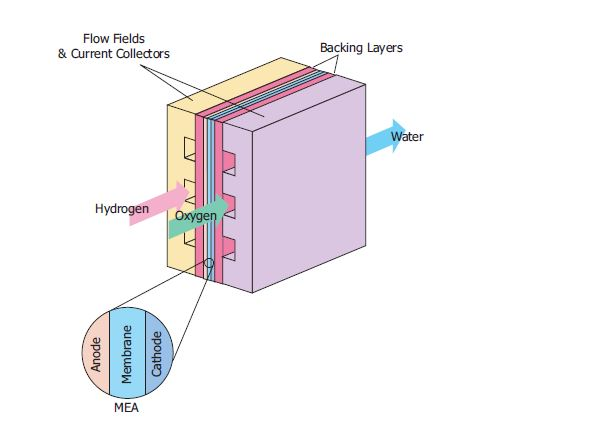
\includegraphics{Figures/Figure3}
%\caption{Fuel Cell Structure
%\cite{pukrushpan_modeling_2003}}
%\end{figure}

\subsection{Problem Statement}
\paragraph{}Monitoring students enterring an institution is an important security step both for the other students as well as for the school property. It is a way to keep off intruders and prevent potential attacks. This monitoring is currently done manually i.e. students have to show their IDs every time they want to enter the school. Another important practice in university education is the signing of sign sheets. This enables the lecturers to keep track of students who attend or don't attend classes. A minimum percentage of classes has to be attained for one to sit for exams.

\paragraph{}These two activities, access control and class attendance, are limited in various aspects. For access control, a student may lose their IDs which will have them refused access into the school despite their frequency there. Also, intruders may use student IDs to access the school. For class attendance, the inaccuracy is due to the prevalent exercise of students signing for their counterparts who do not attend classes. This leaves lecturers at a fix at the end of the semester when they cannot explain low grades among some of their students.

\paragraph{}To solve these two issues, Visage is going to be a face recognition device with attendance generation capabilities. The device will be portable and mountable on the wall.

\subsection{Objectives}
\subsubsection{Main Objective}
To develop a rugged Face recognition device for access control and attendance monitoring
\subsubsection{Specific Objectives}
\begin{enumerate}
\item To design and fabricate a rugged housing for the electronic components of Visage.
\item To build models for Face Recognition.
\item To train the models using data from a given population i.e. volunteers
\item To deploy and showcase Visage at the Tech Expo 12.0
\end{enumerate}

\subsection{Justification of Project}
\paragraph{}\begin{enumerate}
\item Circumstances, like Covid-19, may arise that may need registration of people entering social places e.g. churches. These registrations should not lead to very long queues as was the case previously.
\item Face recognition devices for access control exist but may be expensive. Visage will aim at beingg cost-effective while maintaining or surpassing the efficiency levels.
\item Visage is an opportunity for young African scholars like ourselves to not only learn but also to build using Artificial Intelligence.
\item If Visage is successful it will put JKUAT on the AI map.
\item Employment opportunities for the future for the many data and Machine Learning engineers.
\end{enumerate}

  \clearpage
  %\section{Literature Review}
\subsection{Fuel Cell Operation, Subsystems and Parameters}
\paragraph{}In a (Proton Electron Membrane)PEM fuel cell stack, chemical energy from the reaction between hydrogen and oxygen is converted directly into electric energy. Water and heat are produced as by-products \cite{thanapalan_model_2011}.
\begin{figure}[!h]
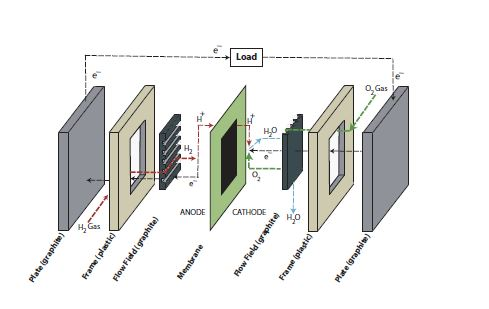
\includegraphics{Figures/Figure5}
\caption{Fuel cell component description
\cite{stefanopoulou_mechatronics_nodate}}
\end{figure} 
\paragraph{}In a hydrogen fuel cell, hydrogen (which we will also refer to as fuel) travels through inlet manifolds to the flow fields. From the flow fields, gas diffuses through porous media to the membrane. The membrane, which is sandwiched in the middle of the cell, contains catalyst and microporous diffusion layers along with gaskets as a single integrated unit. One side of the membrane is  the anode and the other is the cathode. The anode and cathode are more generally referred to as electrodes. The catalyst layer at the anode separates hydrogen molecules into protons and electrons \cite{stefanopoulou_mechatronics_nodate}.
\begin{equation}
$$2H_{2} \rightarrow 4H^{+}+4e^{-}$$
\end{equation}
\paragraph{}The membrane permits only the transfer of  hydrogen protons, requiring the electrons to flow through an external circuit before recombining with protons and oxygen at the cathode-to form water.
\begin{equation}
$$O_{2}+H^{+} + 4e^{-}\rightarrow 2H_{2}O $$
\end{equation}
\paragraph{}The migration of electrons produces electricity. The overall reaction of the fuel cell is:
\begin{equation}
$$2H_{2}+ O_{2} \rightarrow 2H_{2}O+Heat.$$
\end{equation}
\paragraph{}The electrical characteristics of fuel cells are given in the form of a polarization curve, shown in Figure 2.2 , which is a plot of cell voltage versus cell current density (current per unit cell active area) at different reactant pressures and flows.
\begin{figure}[!h]
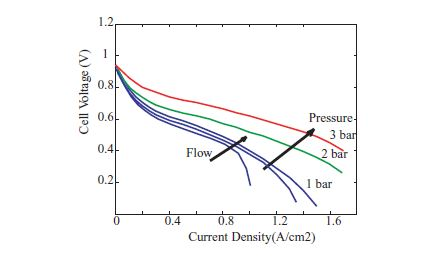
\includegraphics{Figures/Figure6}
\caption{Fuel cell component description
\cite{stefanopoulou_mechatronics_nodate}}
\end{figure}
\paragraph{}Stack temperature and membrane water content affect the fuel cell voltage \cite{ehsani_modern_2018}. The difference between the actual voltage and the ideal voltage represents the loss in the cell which turns into heat. (The ideal standard voltage for a fuel cell in which H2 and O2 react is 1.18 V when the resulting water product is in gaseous form.)
\paragraph{}As more current is drawn from the fuel cell, the voltage decreases, due to fuel cell electrical resistance, low reaction rate and, inefficient reactant gas transport,. Lower voltage indicates lower efficiency of the fuel cell, therefore low load (low current) operation is preferred. Operation at low load requires a large fuel cell stack and has detrimental consequences to the overall volume, weight, and cost.
\paragraph{}To avoid over-sizing the FC stack, a series of actuators such as valves, pumps, blowers, expander vanes, fan motors, humidifiers and condensers are used to control critical FC parameters for a wide range of current, and thus, power setpoints. The auxiliary actuators are needed to make fine and fast adjustments to satisfy reliability standards, performance and safety that are independent of age and operating conditions of the FC. The resulting multivariate design and control synthesis task, also known as balance of plant (BOP), is complex because of subsystem interactions, conflicting objectives, and lack of sensors.
\paragraph{}Main Control among the main FC subsystems are:
\begin{itemize}
\item reactant supply system
\item heating and cooling system
\item humidification system
\item Power management System
\end{itemize}
\paragraph{}The main control variables in FC systems are: 
\begin{itemize}
\item Stack temperature
\item Membrane humidity
\item Accumulation of water and nitrogen in the anode side. 
\end{itemize}
\paragraph{}These variables are the most important factors for any efficiency and lifetime of FC stacks.
\paragraph{}Previous research has concluded that since the fuel cell is a passive power source, a simple feed forward control strategy is used to control the air supply and A PI-feedback algorithm is developed to control the cooling water temperature. The research further concludes that the control strategies need to be further optimized basing on a nonlinear dynamic model.
\begin{figure}[!h]
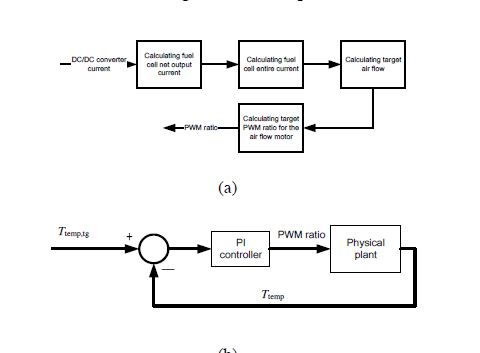
\includegraphics{Figures/Figure8}
\caption{Fuel cell control strategy (a) the air supply system (b) the heat management system
\cite{xu_hierarchical_2010}}
\end{figure}

\paragraph{}Dr. J.T. Pukrushpan et al.\cite{pukrushpan_modeling_2003} studied modelling and control for PEM fuel cell stack
systems, and published several papers. They proposed a nonlinear dynamic model to describe
the PEM fuel cell system, and designed feedback controllers based on the model.
\paragraph{}Further, there have been efforts devoted in controlling the reactant flow system in PEMFCs using only voltage and current measurements and inferring power. More specifically, a single-input
single-output (SISO) controller between the compressor motor voltage and the delivered current or power to the traction motor. Temperature control in available systems is done using large radiators. As a control mechanism to prevent anode flooding, various ingenious mechatronic solutions have been proposed to abate anode flooding (Rodatz et al., 2002)
 \cite{stefanopoulou_mechatronics_nodate}.
\subsection{Fuel Cell Control}
\begin{figure}[!h]
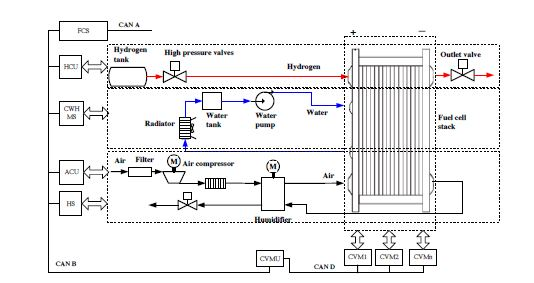
\includegraphics{Figures/Figure7}
\caption{Hydrogen Fuel Cell Control
\cite{xu_hierarchical_2010}}
\end{figure}
\paragraph{}The Fuel cell consists of a hydrogen supply system, a water and heat management system and an air supply system. The compressed hydrogen is stored in several tanks, under  pressures of about 30 MPa. The hydrogen pressure is lowered and kept at a stable level using several valves for safety purposes before the hydrogen goes into the stack. Water accumulates in the stack due to the electrochemical reaction during the operation of the fuel cell, which leads to performance decay. An outlet valve is installed so that the accumulated water can be blown away with hydrogen. The outlet valve and the hydrogen valves used for lowering and stabilizing the pressure are controlled by the Hydrogen Control Unit (HCU).
\paragraph{}The electro-chemical reaction also generates heat, and causes the temperature to increase. The water and heat management system targets to control the stack temperature within a suitable range using deionized water in a water tank. The water flow is controlled by a water pump. The water goes into the stack with a low temperature, and comes out of the stack with a high temperature. A radiator is used to cool the warm water.
\paragraph{}The cooling water temperature is measured, and controlled by a feedback control algorithm.
The air supply system comprises an air filter, a compressor and a humidifier. The impurities in air will cause the catalyst to be poisoned. Thus as a preventive measure, the air should be filtered before getting into the stack. The air flow is controlled by the compressor with a feed forward + feedback algorithm. 
\paragraph{}The air is further humified since there should be some water in the PEM, to allow the PEM to conduct protons. In the humidifier, the dry air is humidified with the damp-heat air out of the stack. The air compressor and the humidifier are controlled by the Air Control Unit (ACU) and the Humidifying System (HS).
\subsection{Summary}
\paragraph{}A fuel cell system integrates many components into a power system. These include DC/DC converters, batteries, and ultracapacitors in the system. In cases where the fuel cell is not fed directly with hydrogen, a reformer must be included. Therefore, there are many control loop schemes, the number of which depends on the configuration of the system. 
\paragraph{}Many control strategies have been proposed in literature, ranging from feed-forward control,Linear quartertic regulator, Neural Networks and Model Predictive Control. A good number of research papers focus on the low level control of the fuel cell to fulfil at least one of the three main objectives such as maximum efficiency, voltage control and/or starvation prevention. However, these designs are still at the theoretical stage and without real time testing. This leads to a methodological gap in the area of hydrogen fuel cell control. The validity of these control strategies for real fuel cell system applications is, however, still under investigation. 
\paragraph{}Furthermore, the extensive studies in the controller design methods are evidence that the fuel cell system control is a very active research area. The research in this area is mainly motivated by the recognition that the current control methods cannot fully meet the desired design requirements on fuel cell system performance, stability, and robustness etc. Any controller design which gives a satisfactory performance on fuel cell system behavior is worth consideration for implementation \cite{ehsani_modern_2018}.


  %\clearpage
   \section{Mechanical Design}
\subsection{Concept Design 1}
\paragraph{Some Design Considerations}
\begin{enumerate}
\item The device should be rugged i.e. it should be able to withstand all weather and conditions.
\item Should be able to house the electronics.
\item Should allow air circulation to prevent the electronics and components from overheating
\item Should have a slot for camera and fan. Fan should further cool the device to minimize chances of overheating.
\item Should provide cheap means of rotational motion.
\end{enumerate}
\paragraph{}Use of sheet metal is one possible option for the device fabrication. Sheet metal is:
\begin{enumerate}
\item Easy to design.
\item Relatively cheap.
\item Able to withstand unfavorable conditions.
\item Readily available.
\end{enumerate} 
\paragraph{}Mild steel is commonly available, but is heavy and easily corroded. Aluminum is light but is expensive. Further research will enable us to choose the metal to use.
\paragraph{} An interim design of Visage housing is shown below.
\begin{center}
\begin{figure}[!h]
\centering
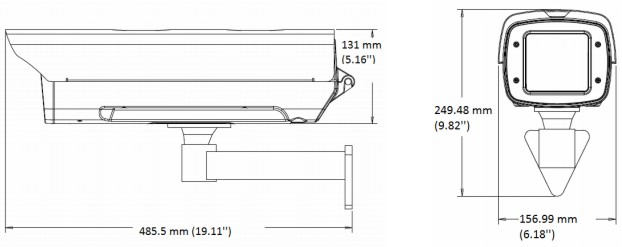
\includegraphics{Figures/Visage}
\caption{Interim Design for Visage using sheet metal}
\end{figure}
\end{center}
\clearpage
\subsection{Conceptual Design 2}

  \clearpage
   \section{Expected Outcomes}
\begin{enumerate}
\item A functional hydrogen stack will be developed and tested
\item The controller for the hydrogen fuel cell will be developed and tested from a selection of controllers that were modelled and simulated.
\item The controller supporting circuitry will be developed with a custom printed circuit board.
\item Hydrogen fuel cell system performance will be optimized using the controller.
\end{enumerate}
\newpage
\section{Proposed Budget}
\begin{table}[!h]
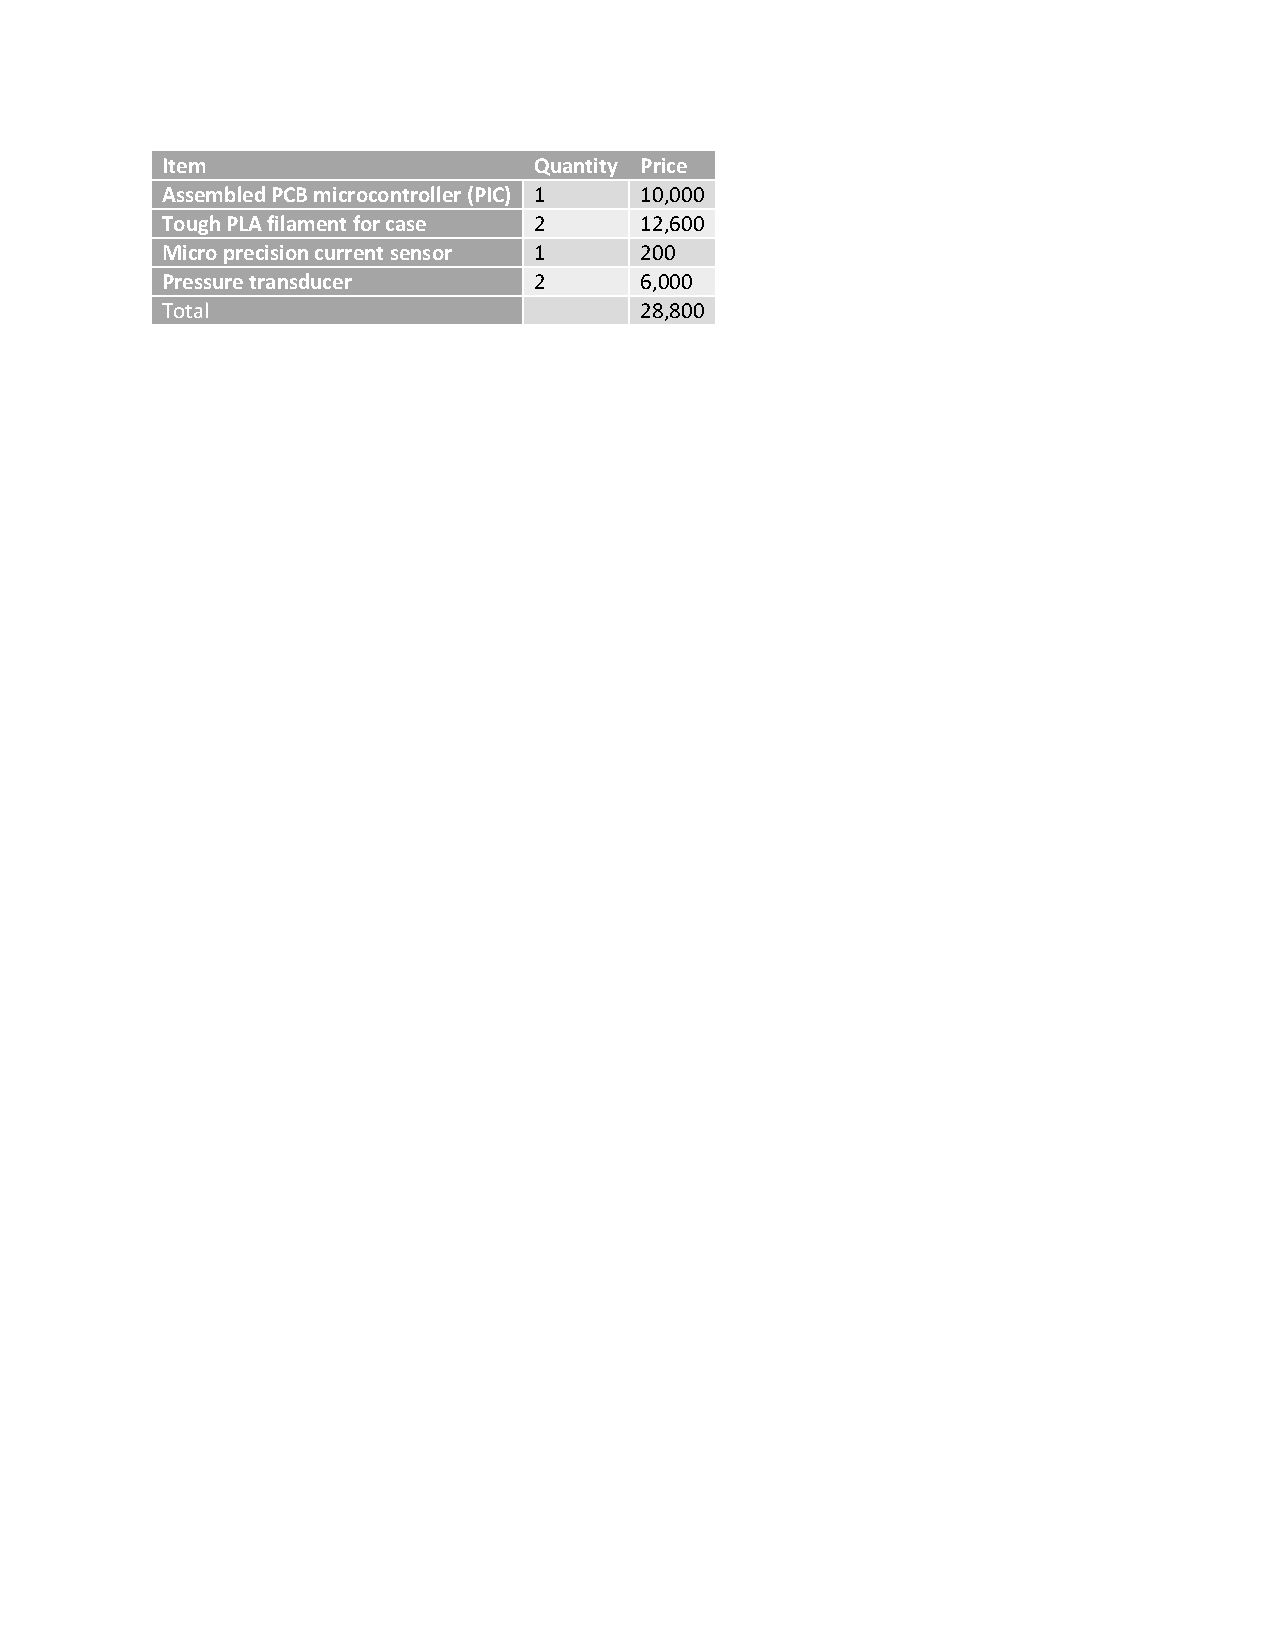
\includegraphics{Figures/budget}
\caption{Proposed budget}
\end{table}
\section{Work Plan}
\begin{table}[!h]
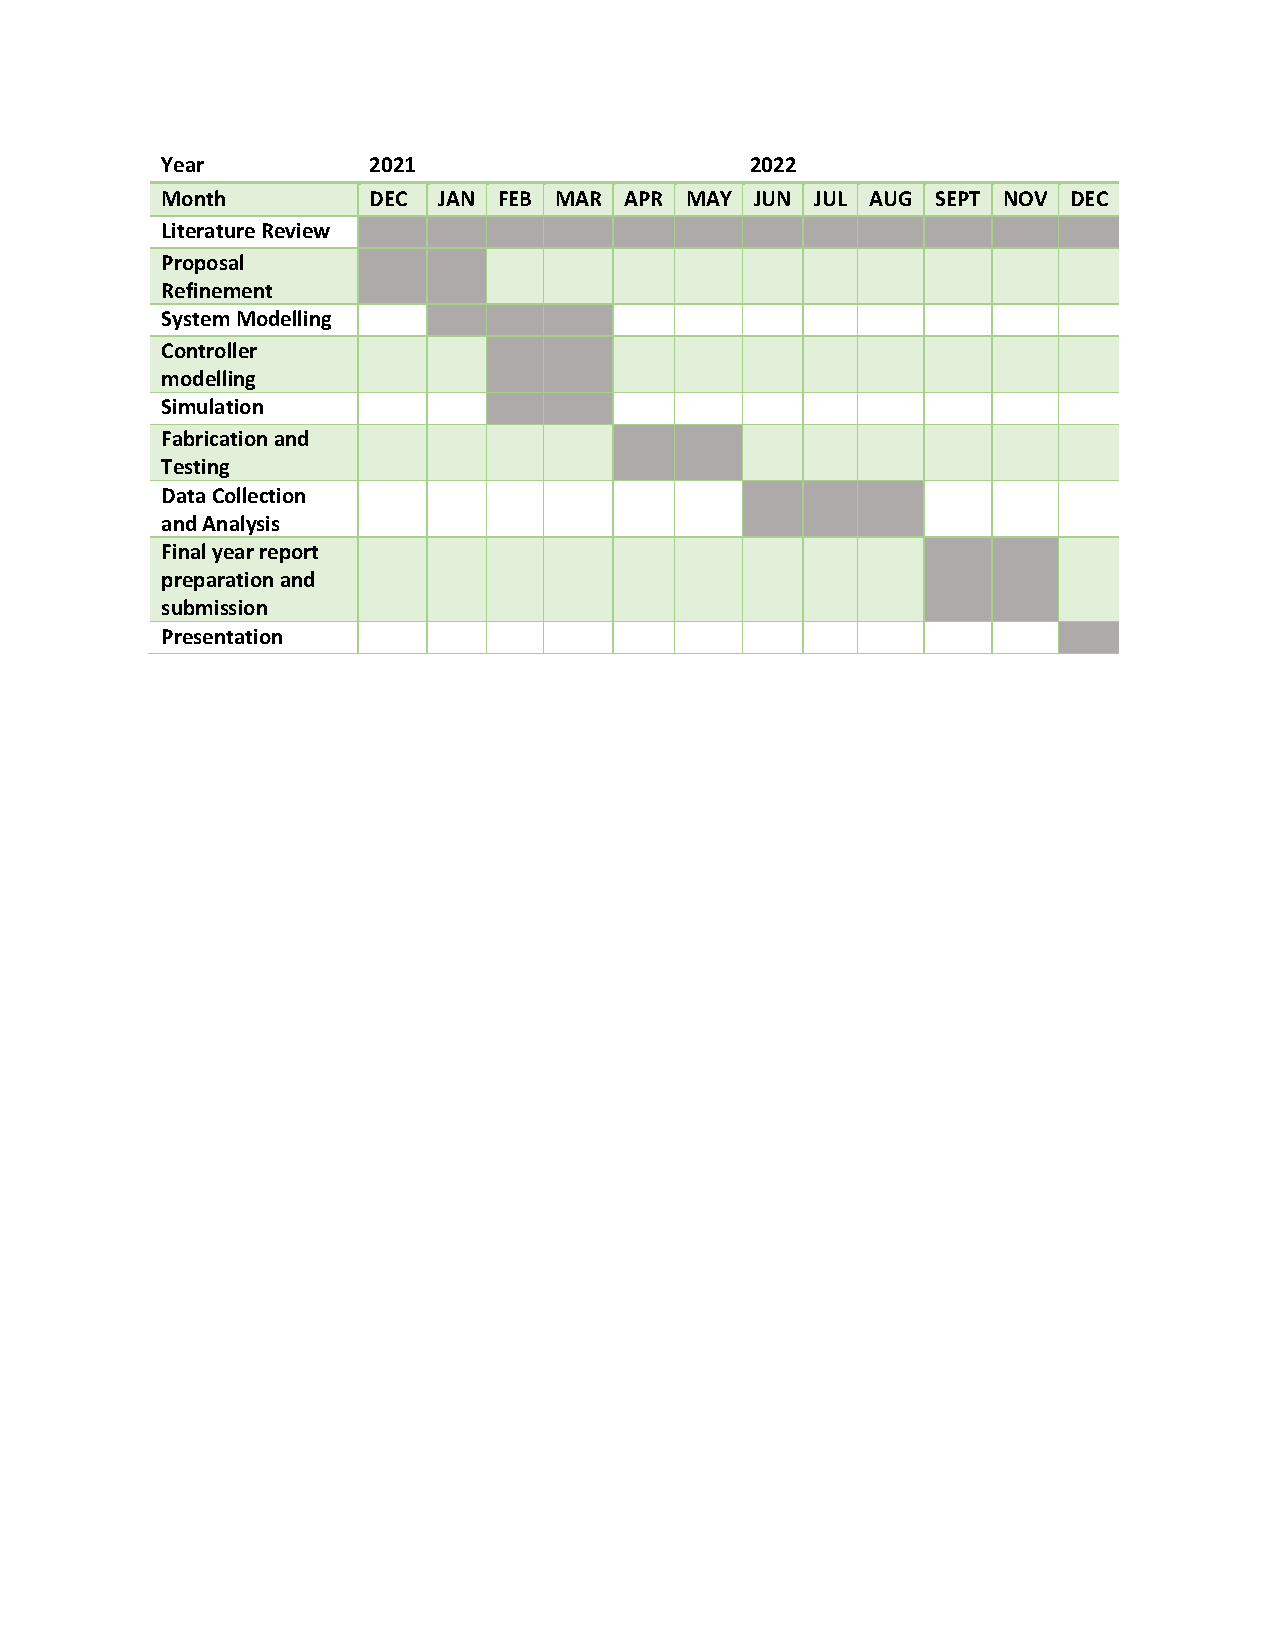
\includegraphics{Figures/workplan}
\caption{Workplan table}
\end{table}

 \clearpage
%  \section{Appendices}
  \clearpage
%----  Bibliography  ----------------------------------------
\markright{References}                               % Erzeugt Kopfzeile
\addcontentsline{toc}{section}{References}            % Literaturverzeichnis ins Inhaltsverzeichnis
\bibliographystyle{Bib/IEEEtran}
\bibliography{Bib/References}                         % BIBTeX
\nocite{Lun01} 

                                     % Falls etwas in die Literaturliste soll, was nicht Referenziert wird
\end{document}
